To further understand how coordination facts work, we present other programs that
take advantage of them.

\subsection{Belief Propagation}

Randomized and approximation algorithms can obtain significant benefits from
coordination directives because although the final program results will not be
exact, they follow important statistical properties and can be computed faster.
An examples of such programs is PageRank~\cite{Lubachevsky:1986:CAA:4904.4801}
and Loopy Belief Propagation~\cite{Gonzalez+al:aistats09paraml}, which is the
focus of this section.

Loopy Belief Propagation (LBP) is an approximate inference algorithm used in
graphical models with cycles~\cite{Murphy99loopybelief}. In its essence, LBP is
a sum-product message passing algorithm where nodes exchange messages with their
immediate neighbors and apply some computations to the messages received.

LBP is an algorithm that maps very well to the graph-based model of LM. The
original algorithm computes the belief of all nodes for several iterations with
synchronization between iterations. However, it is possible to avoid the
synchronization step, if we take advantage of the fact that LBP will converge
even when using an asynchronous approach. So, instead of computing the belief
iteratively, we keep track of all messages sent/received (and overwrite them
when we receive a new one) and recompute the belief asynchronously. In our
particular implementation, the graph of nodes is a grid where each node
represents a pixel and we are trying to de-noise an image.
Figure~\ref{fig:coordination:bp} shows the communication patterns for our
application and Fig.~\ref{code:coordination:bp} presents the LM code for the
implementation.

\begin{figure}[h]
   \begin{center}
      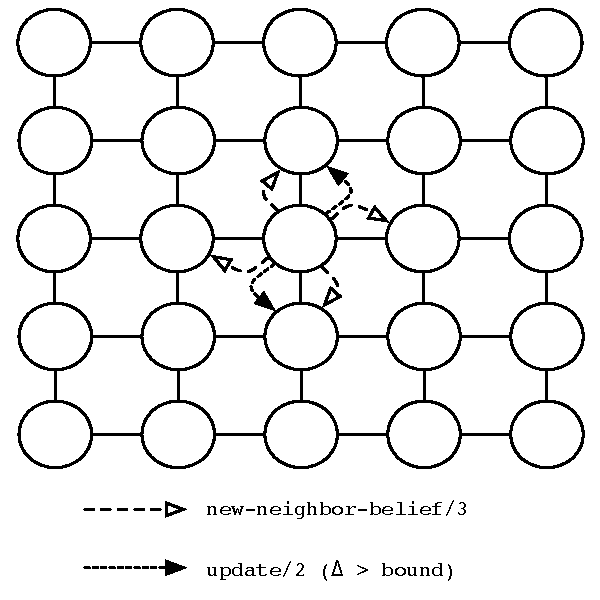
\includegraphics[width=0.3\textwidth]{figures/bp/bp.pdf}
   \end{center}
\caption{LBP: communication patterns}
\label{fig:coordination:bp}
\end{figure}


\begin{figure}[h!]
\small\begin{Verbatim}[numbers=left]
neighbor-belief(A, B, Belief),
new-neighbor-belief(A, B, NewBelief)
   -o neighbor-belief(A, B, NewBelief).

check-residual(A, Residual, B),
Residual > bound
   -o update(B).
check-residual(A, _, _) -o 1.

// update belief to be sent to one neighbor
update-messages(A, NewBelief),
!edge(A, B),
neighbor-belief-old(A, B, OldIn),
sent-neighbor-belief(A, B, OldOut),
Cavity = normalize(divide(NewBelief, OldIn)),
Convolved = normalize(convolve(global-potential, Cavity)),
OutMessage = damp(Convolved, OldOut, damping)
   -o Residual = residual(OutMessage, OldOut),
      check-residual(A, Residual, B),
      update-messages(A, NewBelief),
      new-neighbor-belief(B, A, OutMessage),
      sent-neighbor-belief(A, B, OutMessage).

update-messages(A, NewBelief) -o 1.

// if we have two update functions, just run one of them
update(A), update(A) -o update(A).

// make a copy of neighbors beliefs in order to add them up
update(A),
!potential(A, Potential),
belief(A, MyBelief)
   -o [custom addfloats Potential => Belief | B, Belief, Normalized | neighbor-belief(A, B, Belief) |
            neighbor-belief-old(A, B, Belief), neighbor-belief(A, B, Belief) |
            Normalized = normalizestruct(Belief), update-messages(A, Normalized), belief(A, Normalized)].
\end{Verbatim}
\caption{LM program for the Loopy Belief Propagation problem}
\label{code:coordination:bp}
\end{figure}

Belief values are lists of floats and are represented by \texttt{belief/2}
facts. The first rule (lines 1-2) updates a given neighbor belief whenever a new
belief value is received. This is the highest priority rule since we want to
update the neighbor beliefs before doing anything else. In order to store the
belief values of the neighbor nodes, we use \texttt{neighbor-belief/3} facts,
where the second argument is the neighbor address and the third argument is the
belief value.

The last two rules (lines 24-29) update the belief value of a node. An
\texttt{update/1} fact starts the process. The first rule (lines 24-25) simply
consumes redundant \texttt{update/1} facts and the second rule (lines 26-29)
consumes a node's \texttt{belief/2} fact and derives copies of the neighbors
beliefs, that are going to be used to derive the new belief value, and a
\texttt{sum-messages/2} fact, used to accumulate the neighbors belief values.
The rule in lines 4-5 consumes a neighbor belief value to update the
\texttt{sum-messages/2} fact and the rule in lines 6-7 derives the new belief
value. Since the rule in lines 4-5 has higher priority, it will be applied as
long as we have neighbor belief values (\texttt{neighbor-belief-copy/2}) to
consume. Only then the rule in lines 6-7 will finally derive the new belief
value.

Once the neighbor belief values are added up, we use the accumulated value to
send new belief information to our neighbors (rules in lines 15-24). Again, we
use rule priorities to go first through all the neighbors (rule in lines 15-20),
before consuming \texttt{update-messages/2} facts (rule in lines 21-22). We also
compute the delta of the belief value we sent previously using the
\texttt{residual/2} function (line 18), so that we can decide if that specific
neighbor node should recompute its belief value. This is done in rule in lines
9-10 by comparing \texttt{Delta} with a pre-defined \texttt{bound} constant
value. When that is the case, we simply derive \texttt{update(B)} at the
neighbor node \texttt{B} (line 10).

The above algorithm is highly asynchronous, therefore it fits well with the
concurrent nature of LM.
